\documentclass[a4paper,12pt]{article}
\setlength{\headheight}{68.803pt}
\addtolength{\topmargin}{-56.803pt}

\usepackage[utf8]{inputenc}
\usepackage[T1]{fontenc}
\usepackage{lmodern}
\usepackage[nopatch=footnote]{microtype}
\usepackage{fvextra}
\DefineVerbatimEnvironment{Verbatim}{Verbatim}{
  breaklines=true,
  breakanywhere=true,
  frame=single,
  fontsize=\small
}

% margin settings
\usepackage[
  left=1in,
  right=1in,
  top=3cm,
  bottom=1in
]{geometry}

\usepackage[
    colorlinks=true,
    linkcolor=black,
    urlcolor=blue,
    citecolor=blue,
    pdfborder={0 0 0},
    pdfauthor={Massimo Mantineo},
    pdftitle={ICMP con Socket Raw},
    pdfsubject={Laboratorio di Reti e Sistemi Distribuiti: HANDS-ON 5},
]{hyperref}

\usepackage{graphicx}
\graphicspath{{../../assets/}}
\usepackage{tikz}
\usetikzlibrary{positioning, arrows.meta, shapes.symbols}
\usepackage{listings}
\usepackage{xcolor}
\usepackage{amsmath, amssymb}
\usepackage{fancyhdr}
\usepackage{setspace}
\usepackage{pgfplots}
\pgfplotsset{compat=1.17}
\usepackage{booktabs}
\usepackage[skins, listings]{tcolorbox}
\usepackage{float}

\newtcblisting{terminal}[1][]{
    listing only,
    colback=black!85!white,
    colframe=black!70!white,
    colupper=green!80!white,
    coltitle=white,
    title=#1,
    fonttitle=\bfseries\sffamily,
    listing options={
        language={},
        basicstyle=\ttfamily\small\color{green!80!white},
        backgroundcolor={},
        frame=none,
        breaklines=true,
        showstringspaces=false,
        numbers=none
    },
    enhanced,
    drop shadow,
    arc=3mm
}

\newtcblisting{ccode}[1][]{
    listing only,
    colback=blue!3!white,
    colframe=blue!70!black,
    title=#1,
    fonttitle=\bfseries\sffamily,
    listing options={
        style=cstyle,
        backgroundcolor={},
        frame=none
    },
    enhanced,
    drop shadow,
    arc=3mm
}

\setlength{\footskip}{50pt}

% settings for C listings
\lstdefinestyle{cstyle}{
    language=C,
    basicstyle=\ttfamily\small,
    numbers=left,
    numberstyle=\tiny,
    stepnumber=1,
    numbersep=5pt,
    backgroundcolor=\color{white},
    showspaces=false,
    showstringspaces=false,
    showtabs=false,
    frame=single,
    tabsize=4,
    captionpos=b,
    breaklines=true,
    breakatwhitespace=true,
    keywordstyle=\color{blue}\bfseries,
    commentstyle=\color{green!50!black},
    stringstyle=\color{red},
}
\lstset{style=cstyle}

% Header and Footer
\pagestyle{fancy}
\fancyhf{}

\fancyhead[L]{%
  \parbox[b]{0.45\textwidth}{%
    \small
    Student Name: Massimo Mantineo\\
    Student ID: 541924
    \vspace{20pt}
  }%
}
\fancyhead[C]{%
  \parbox[b]{0.2\textwidth}{%
    \centering
    \normalsize \bfseries
    LabReSiD25\\
    Hands-On 5
    \vspace{20pt}
  }%
}
\fancyhead[R]{%
  \parbox[b]{0.35\textwidth}{%
    \flushright
    \includegraphics[width=3.5cm]{\detokenize{logo_unime_orizontale.png}}
    \vspace{15pt}
  }%
}

\renewcommand{\contentsname}{Indice}

\title{\vspace{-2cm}Relazione: Implementazione ICMP con Socket Raw\\
\large (Hands-On 5)}
\author{Massimo Mantineo \\ Matricola: 541924}
\date{MESSINA, A.A. 2024/2025}

\begin{document}

% Cover page
\begin{titlepage}
    \thispagestyle{empty}
    \centering
    \vspace*{1cm}
    \includegraphics[width=6cm]{\detokenize{logo_unime_orizontale.png}}\par\vspace{1cm}
    \vspace{2cm}
    {\Large \textbf{Università degli Studi di Messina}\par}
    {\large Dipartimento MIFT - Corso di Laurea Triennale in Informatica (L-31)\par}
    \vspace*{1cm}
    {\large Laboratorio di Reti e Sistemi Distribuiti\par}
    \vspace{1cm}
    {\Large \textbf{HANDS-ON 5:}\\
    Analisi e Implementazione ICMP con Socket Raw\par}
    \vspace{2cm}
    {\large Massimo Mantineo \par}
    {\large Matricola: 541924 \par}
    \vfill
    {\large Messina, A.A. 2024/2025 \par}
\end{titlepage}

\clearpage
\pagestyle{fancy}
\tableofcontents
\newpage

\section{Problem Statement}
L'obiettivo della quinta esercitazione (Hands-On 5) è lo studio e l'implementazione del protocollo **ICMP** (\textit{Internet Control Message Protocol}) tramite l'impiego dei **Socket Raw**. L'attività consiste nel progettare un applicativo C capace di generare pacchetti \textit{Echo Request} (Ping) personalizzati, bypassando gli stack di trasporto standard (TCP/UDP) del kernel. La sfida tecnica risiede nella gestione manuale dell'incapsulamento IP, nel calcolo del checksum secondo gli standard RFC e nel parsing accurato della risposta catturata dallo stream di bit grezzi proveniente dalla rete.

\section{Stato dell'Arte}
Il protocollo ICMP (RFC 792) è lo strumento fondamentale per la diagnostica e il controllo degli errori nelle reti IP.
\begin{itemize}
    \item \textbf{Struttura del Messaggio}: Un pacchetto ICMP è composto da un header di 8 byte (Tipo, Codice, Checksum, Identificatore e Numero di Sequenza) seguito da un payload opzionale.
    \item \textbf{Socket Raw (\texttt{SOCK_RAW})}: A differenza dei socket tradizionali, i socket raw permettono l'accesso diretto ai protocolli del livello di rete. L'uso di \texttt{IPPROTO_ICMP} istruisce il kernel a non aggiungere header di trasporto, delegando all'applicazione la costruzione del pacchetto. Per ragioni di sicurezza, queste operazioni richiedono privilegi di amministrazione (\texttt{root/sudo}).
    \item \textbf{Endianness}: Poiché i campi dell'header (come l'Identifier) sono multi-byte, è essenziale gestire la conversione tra l'ordine dei byte dell'host (Little-Endian su x86) e quello della rete (Big-Endian) tramite \texttt{htons()} e \texttt{ntohs()}.
\end{itemize}

\section{Metodologia ed Implementazione}
L'implementazione si articola nella costruzione del pacchetto e nell'analisi della risposta tramite aritmetica dei puntatori.

\subsection{Costruzione del Pacchetto Echo Request}
Viene allocato un buffer in cui si mappano le strutture \texttt{struct icmphdr}. Il checksum deve essere calcolato sull'intero header ICMP e sul payload prima dell'invio.
\begin{ccode}[Snippet Calcolo Checksum ICMP]
unsigned short compute_checksum(void *addr, int len) {
    int sum = 0; unsigned short *ptr = addr;
    while (len > 1) { sum += *ptr++; len -= 2; }
    if (len == 1) sum += *(unsigned char *)ptr;
    sum = (sum >> 16) + (sum & 0xFFFF);
    sum += (sum >> 16);
    return (unsigned short)(~sum);
}
\end{ccode}

\subsection{Ricezione e Parsing IP}
Al momento della ricezione, il kernel restituisce anche l'header IP (20 byte). È necessario estrarre la lunghezza dell'header IP (\texttt{ihl}) per individuare l'inizio del payload ICMP:
\begin{ccode}[Snippet Parsing Risposta]
struct iphdr *ip_hdr = (struct iphdr *)recv_buffer;
// L'header ICMP inizia dopo (IHL * 4) byte
struct icmphdr *icmp_reply = (struct icmphdr *)(recv_buffer + (ip_hdr->ihl * 4));
\end{ccode}


\subsection{Istruzioni di Esecuzione}
L'uso dei raw socket richiede privilegi elevati (sudo):
\begin{terminal}[Build & Run]
$ gcc ICMP_raw.c -o icmp_ping
$ sudo ./icmp_ping 8.8.8.8
\end{terminal}

\section{Risultati}
La validazione è stata condotta interrogando il server DNS di Google (\texttt{8.8.8.8}) con privilegi di \texttt{root}.

\begin{figure}[H]
    \centering
    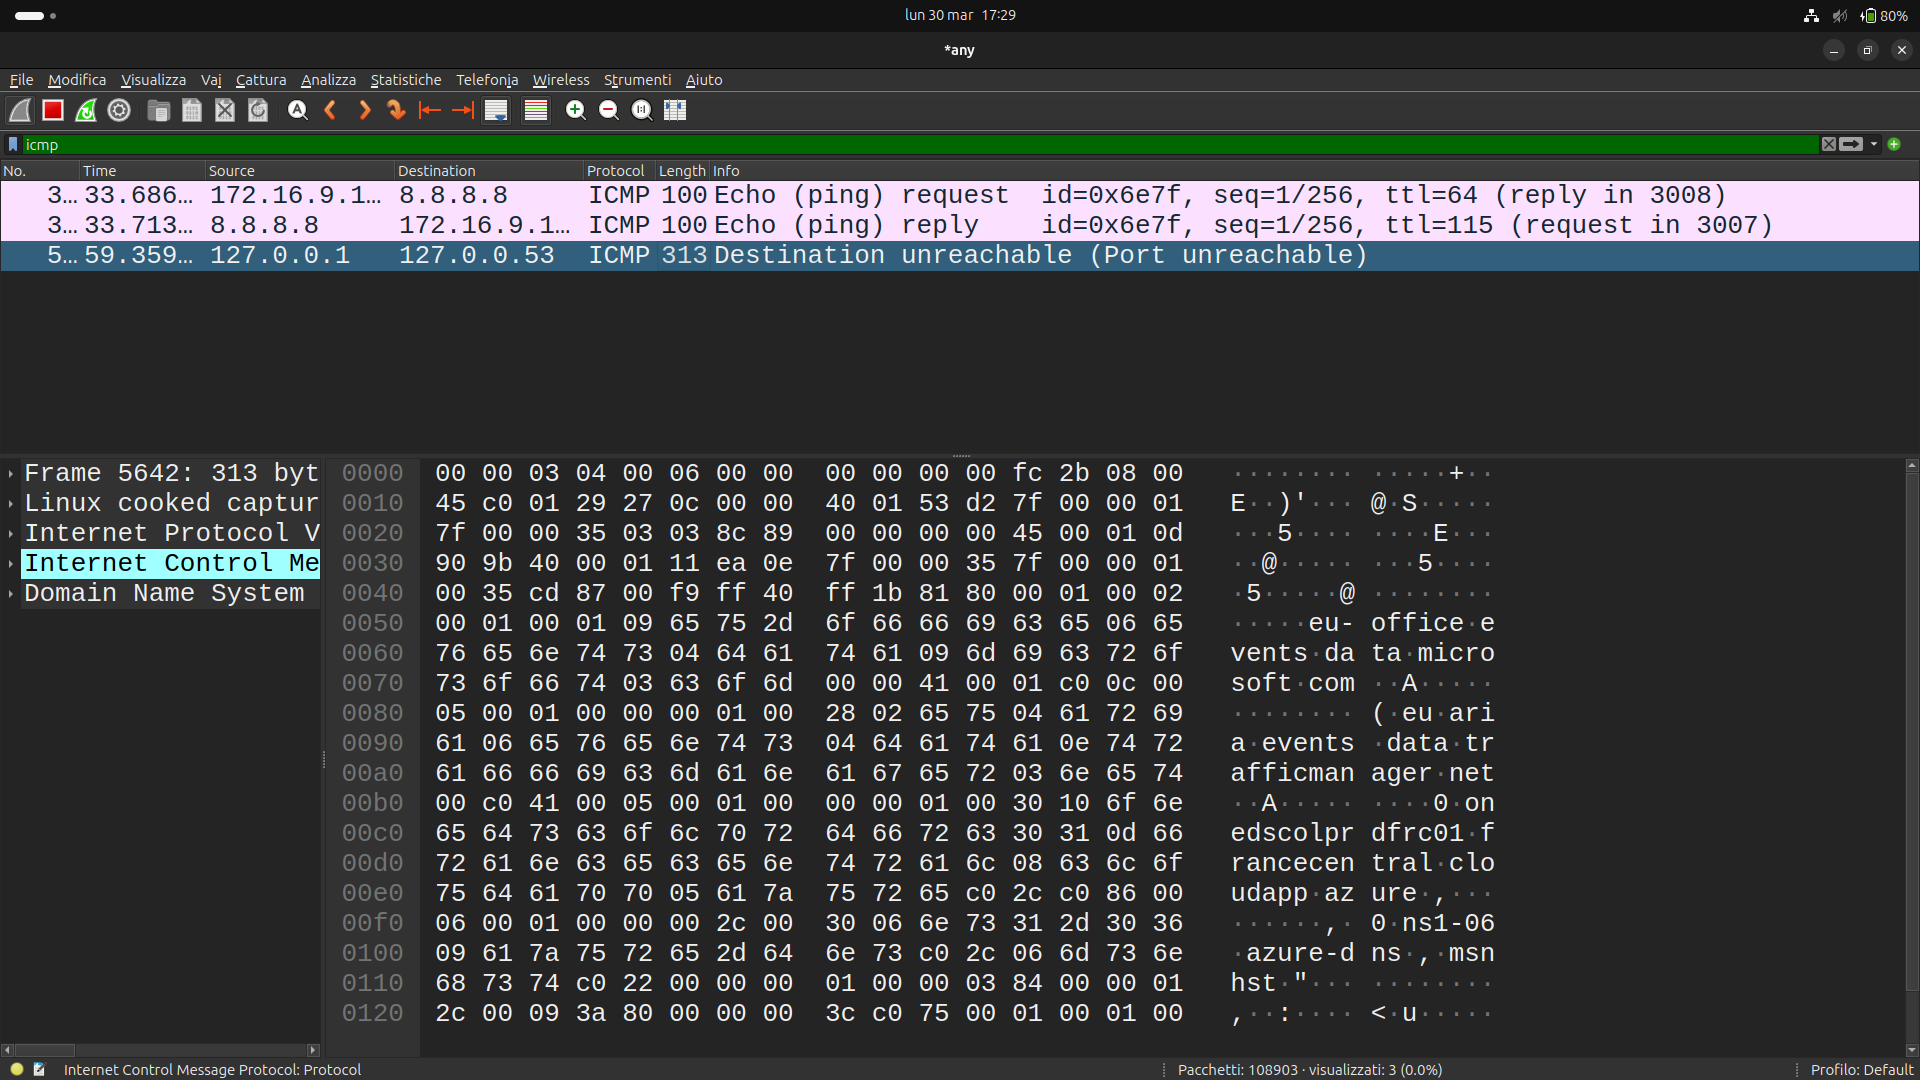
\includegraphics[width=0.9\textwidth]{ho5/ho5_icmp_request.png}
    \caption{Cattura pacchetti ICMP su Wireshark.}
    \label{fig:icmp_capture}
\end{figure}

\subsection{Test di Raggiungibilità}
Il programma ha riportato con successo la ricezione dell'Echo Reply (Tipo 0), confermando il corretto matching tra l'ID del processo e l'ID contenuto nel pacchetto di ritorno.
\begin{terminal}[Output Ping Custom]
$ sudo ./icmp_ping 8.8.8.8
Invio ICMP Echo Request (id=1234, seq=1)...
Ricevuta risposta: seq=1, TTL=117, bytes=64
\end{terminal}

\subsection{Analisi Wireshark}
L'ispezione della cattura (Figura 5) conferma che il payload personalizzato 'AAAA' (\texttt{0x41}) è stato correttamente incapsulato e restituito dal server remoto, validando la funzione di checksum.

\section{Conclusioni e Sviluppi Futuri}
L'Hands-On 5 ha permesso di comprendere l'anatomia dei protocolli di controllo e il potere derivante dall'accesso diretto al network stack tramite socket raw. Questa competenza è la base per lo sviluppo di tool di scansione e monitoraggio professionale.

\noindent \textbf{Sviluppi futuri:}
\begin{itemize}
    \item \textbf{Traceroute}: Implementazione di un tool di tracciamento rotta manipolando il campo \texttt{TTL} (Time-To-Live) dell'header IP per indurre errori di \textit{Time Exceeded}.
    \item \textbf{ICMPv6}: Adattamento del codice per lo stack IPv6, analizzando le differenze nella gestione del Checksum (che in IPv6 include uno pseudo-header IP).
\end{itemize}

\end{document}
